\documentclass[12pt,letterpaper]{article}
\usepackage[utf8]{inputenc}
\usepackage[T1]{fontenc}
\usepackage[activeacute,spanish]{babel}
\usepackage[left=18mm,right=18mm,top=21mm,bottom=21mm,letterpaper]{geometry}%
\usepackage{helvet}
\usepackage{amsmath,amsfonts,amssymb,commath}
\usepackage{graphicx}
\usepackage{color}
\usepackage{xcolor}
\usepackage{verbatim}
\usepackage{tabls}
\usepackage[space]{grffile}
\usepackage{url}
\usepackage{listings}
\usepackage{circuitikz}
\usepackage{siunitx}

\usepackage{matlab-prettifier}

\usepackage{textcomp}
\usepackage{booktabs}
\usepackage[colorlinks=true,urlcolor=blue,linkcolor=black,citecolor=black]{hyperref} 
\usepackage{pdfpages}   %incluir paginas de pdf externo, para los anexos
\usepackage{caption}
\usepackage{subcaption}  
\usepackage{rotating}
\usepackage[section]{placeins}
\usepackage{tikz}

\begin{document}

\title{Laboratorio 2 MATLAB}
\author{Daniel García Vaglio (B42781), Esteban Zamora (B47769), Ariel Fallas (B42481)}
\maketitle

\section{Ejercico 1}
En el primer ejercicio se hace primero la simulación con las condiciones iniciales descritas. 


%Primera simulacion ···········································································································································
\begin{figure}
	\centering
	\begin{subfigure}[b]{0.36\textwidth}
		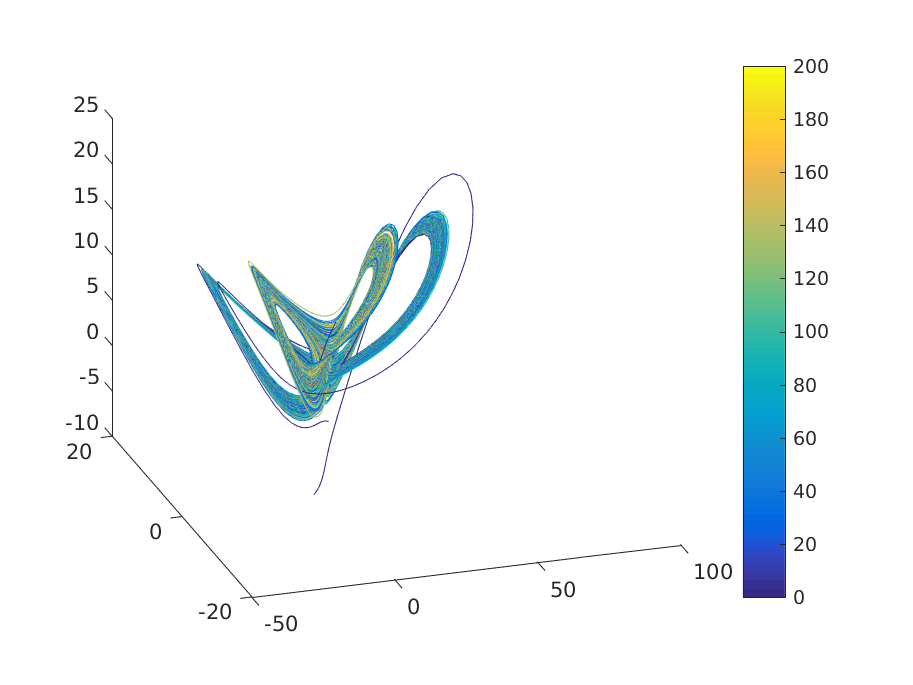
\includegraphics[width=\textwidth]{pictures/primera_simulacion}
		\caption{Resultado para primer caso de condiciones ininciales}
		\label{fig:simulacion1}
	\end{subfigure}
	\begin{subfigure}[b]{0.36\textwidth}
		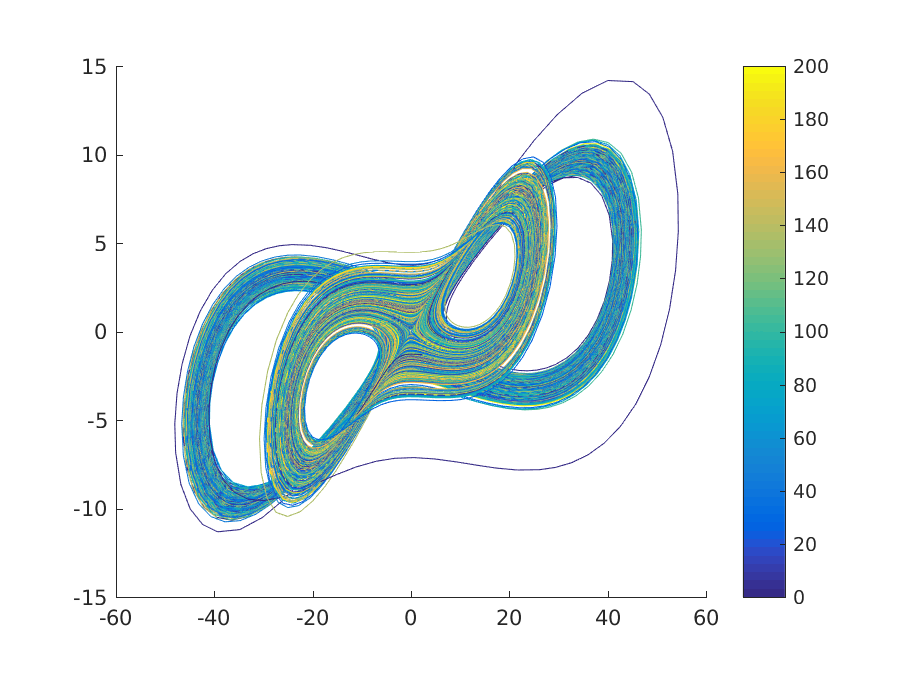
\includegraphics[width=\textwidth]{pictures/primera_simulacion_xy}
		\caption{Vista XY de la primera simulación}
		\label{fig:simulacion1xy}
	\end{subfigure}
        \vfill
        \begin{subfigure}[b]{0.36\textwidth}
		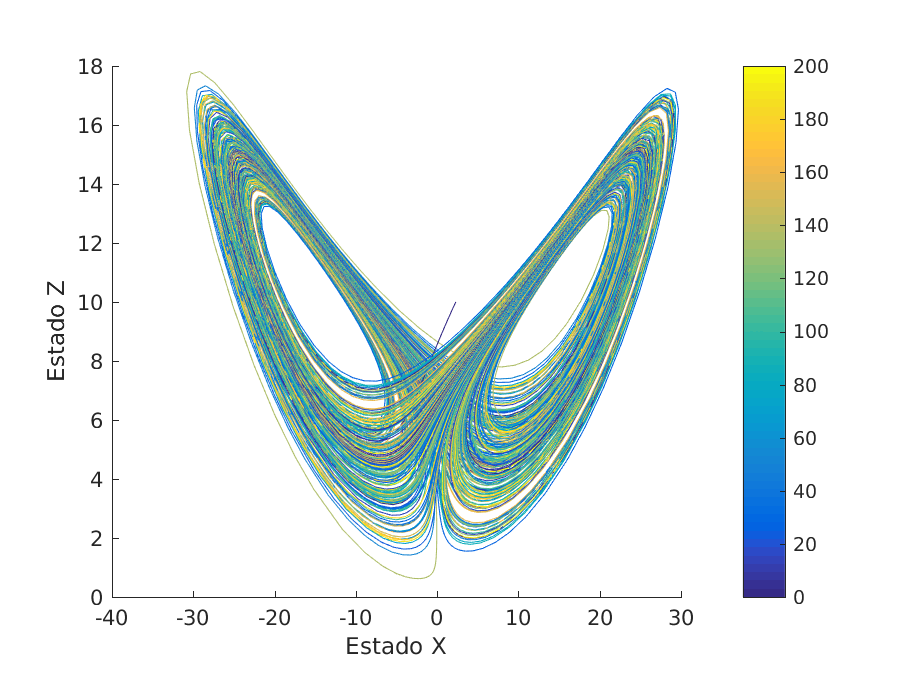
\includegraphics[width=\textwidth]{pictures/primera_simulacion_xz}
		\caption{Vista XZ de la primera simulación}
		\label{fig:simulacion1xz}
	\end{subfigure}

        \begin{subfigure}[b]{0.36\textwidth}
		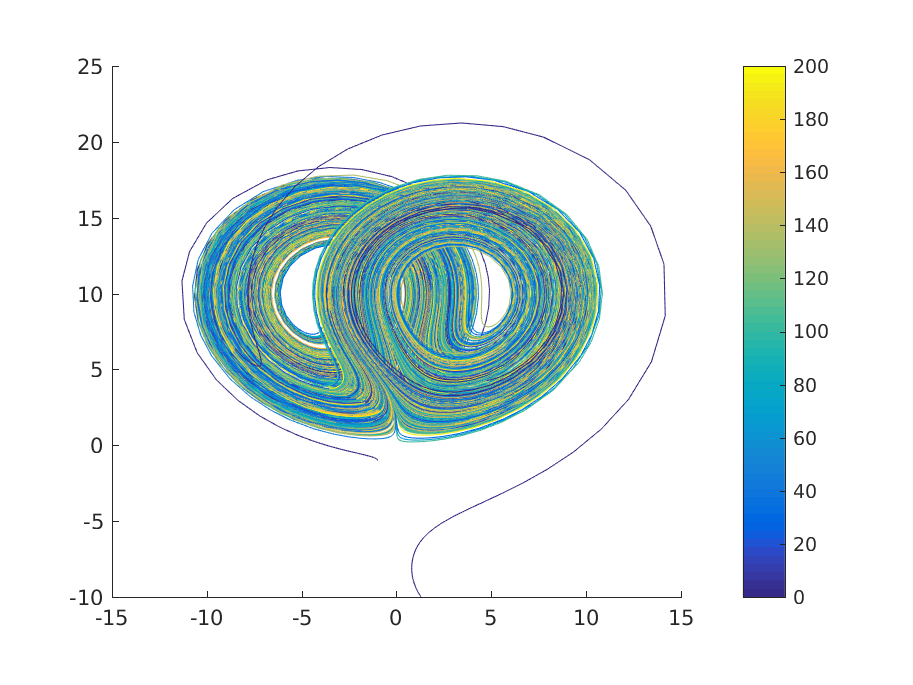
\includegraphics[width=\textwidth]{pictures/primera_simulacion_yz}
		\caption{Vista YZ de la primera simulación}
		\label{fig:simulacion1yz}
	\end{subfigure}
	\caption{Primera simulación gráfica de los estados. En los ejes se tienen los estados y el tiempo se denota con el cambio de color}
	\label{fig:simulacion1_total}
\end{figure}

%segunda simulacion ···········································································································································
\begin{figure}
	\centering
	\begin{subfigure}[b]{0.36\textwidth}
		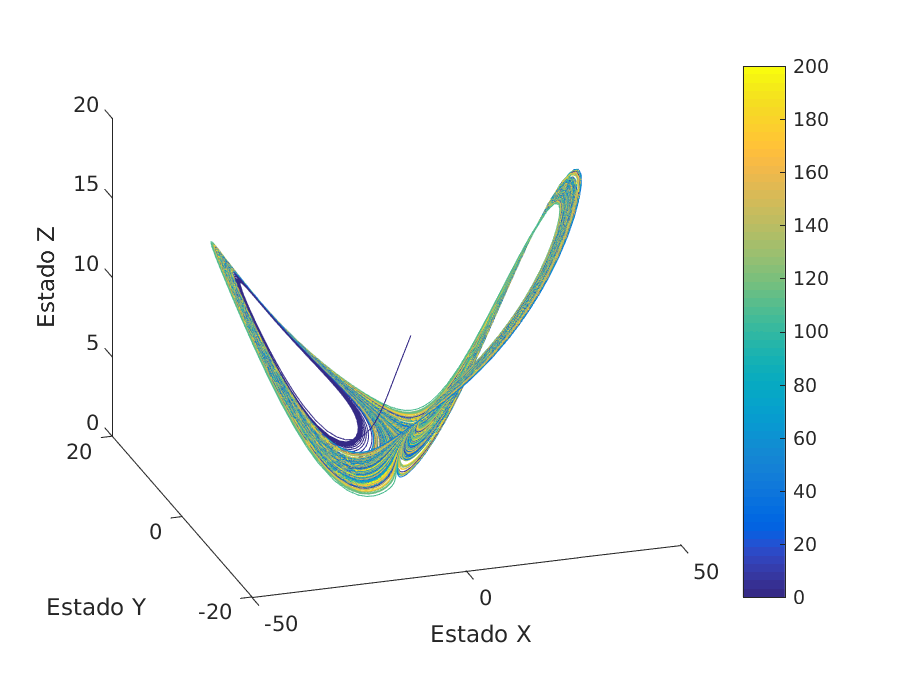
\includegraphics[width=\textwidth]{pictures/segunda_simulacion}
		\caption{Resultado para primer caso de condiciones ininciales}
		\label{fig:simulacion2}
	\end{subfigure}
	\begin{subfigure}[b]{0.36\textwidth}
		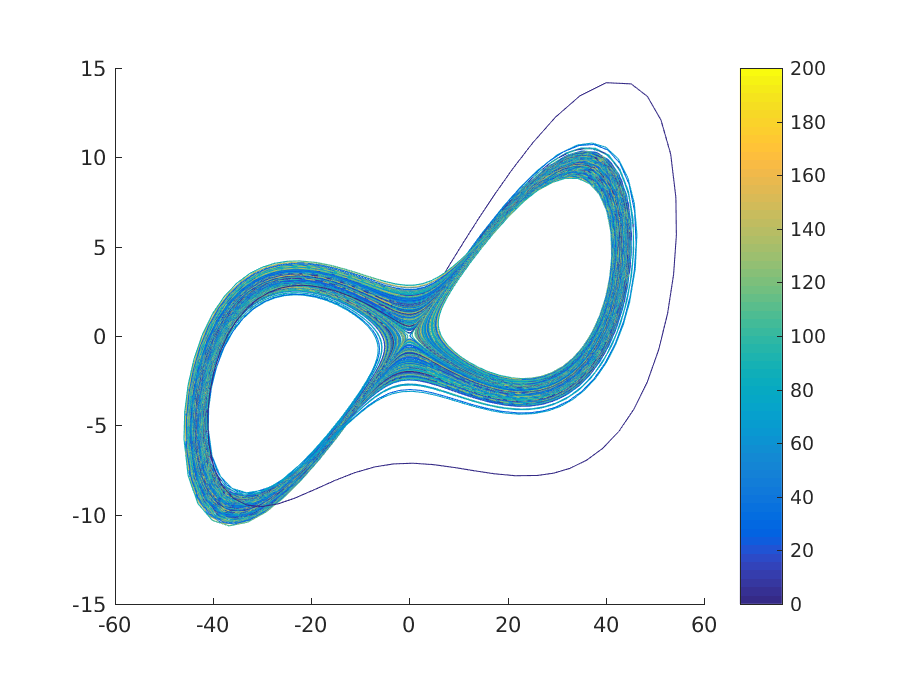
\includegraphics[width=\textwidth]{pictures/segunda_simulacion_xy}
		\caption{Vista XY de la segunda simulación}
		\label{fig:simulacion2xy}
	\end{subfigure}
        \vfill
        \begin{subfigure}[b]{0.36\textwidth}
		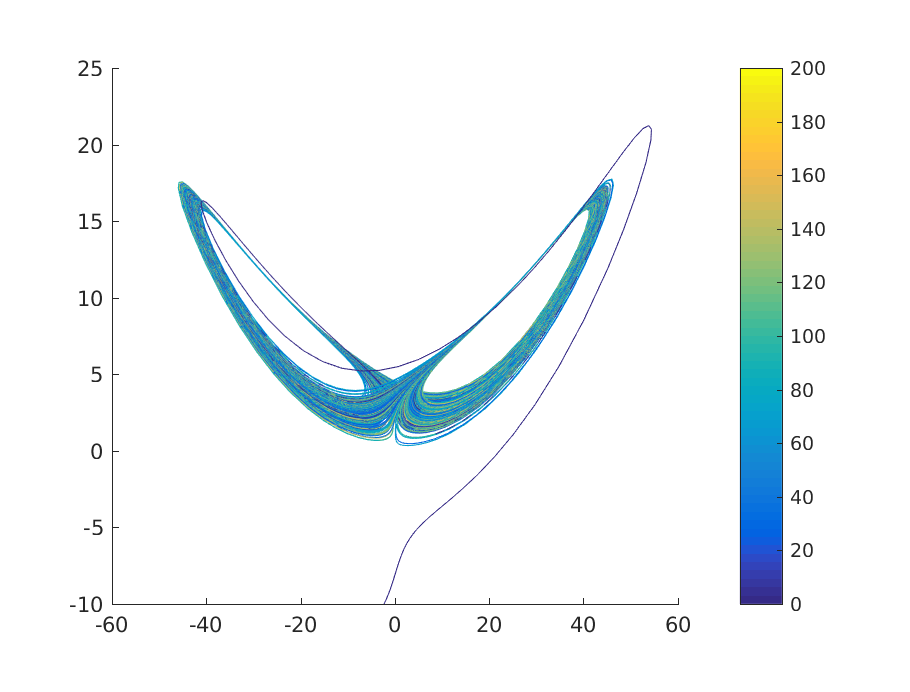
\includegraphics[width=\textwidth]{pictures/segunda_simulacion_xz}
		\caption{Vista XZ de la segunda simulación}
		\label{fig:simulacion2xz}
	\end{subfigure}

        \begin{subfigure}[b]{0.36\textwidth}
		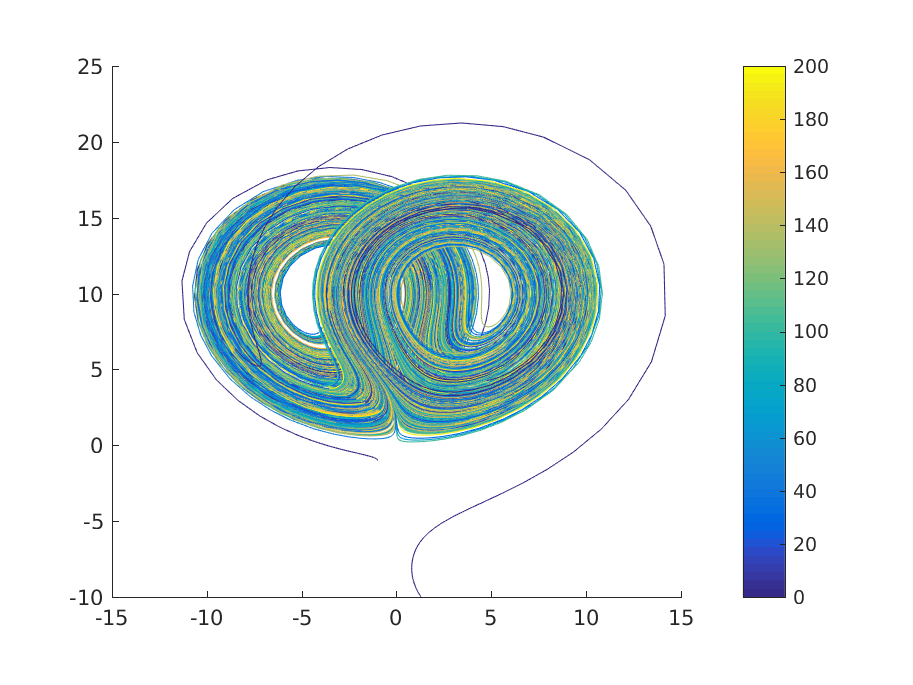
\includegraphics[width=\textwidth]{pictures/segunda_simulacion_yz}
		\caption{Vista YZ de la segunda simulación}
		\label{fig:simulacion2yz}
	\end{subfigure}
	\caption{Segunda simulación gráfica de los estados. En los ejes se tienen los estados y el tiempo se denota con el cambio de color}
	\label{fig:simulacion2_total}
\end{figure}

%Tercera simulacion ···········································································································································

\begin{figure}
	\centering
	\begin{subfigure}[b]{0.36\textwidth}
		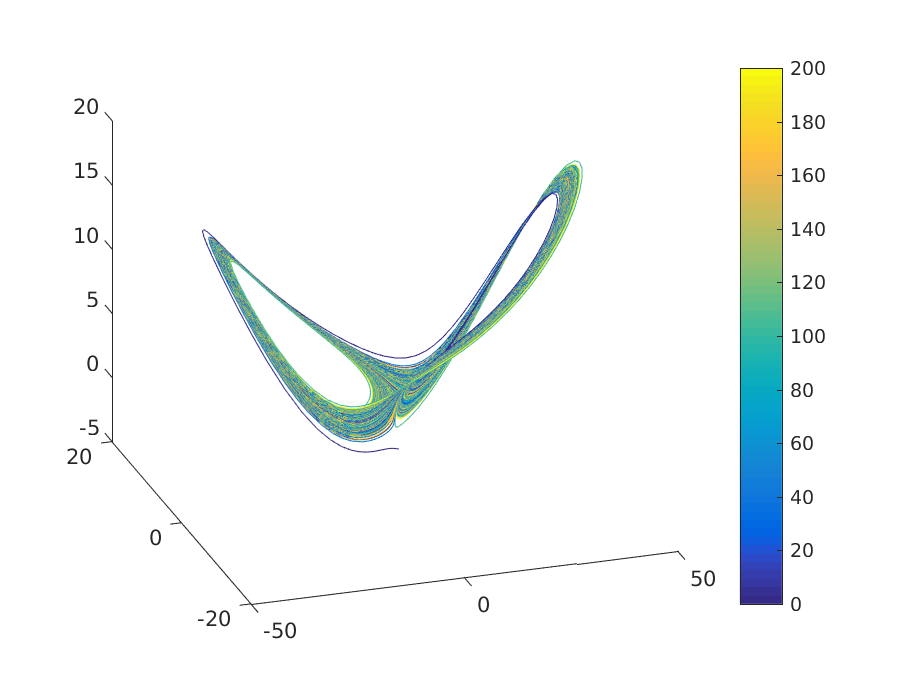
\includegraphics[width=\textwidth]{pictures/tercera_simulacion}
		\caption{Resultado para primer caso de condiciones ininciales}
		\label{fig:simulacion3}
	\end{subfigure}
	\begin{subfigure}[b]{0.36\textwidth}
		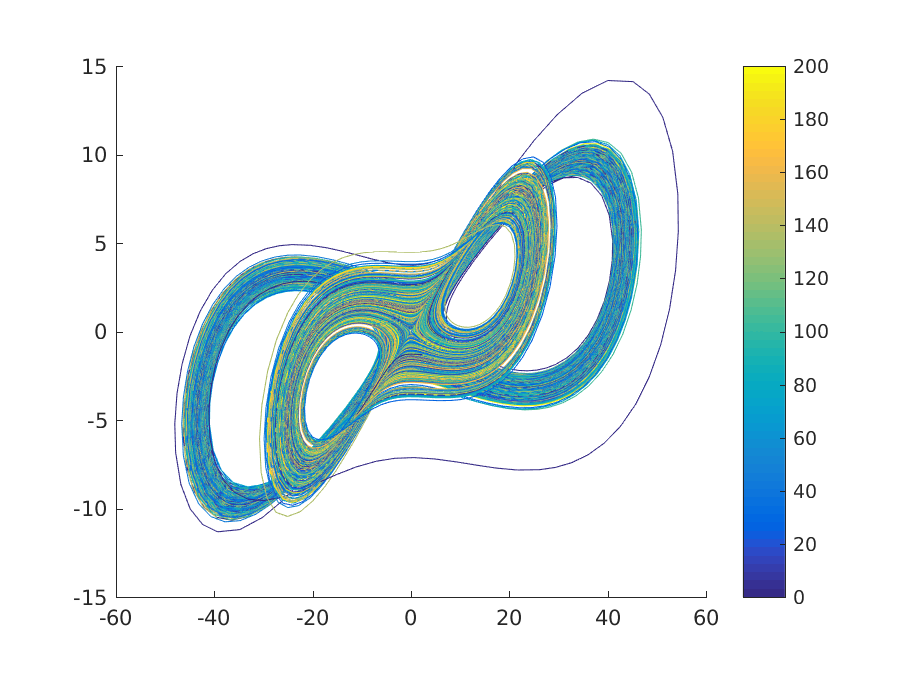
\includegraphics[width=\textwidth]{pictures/tercera_simulacion_xy}
		\caption{Vista XY de la tercera simulación}
		\label{fig:simulacion3xy}
	\end{subfigure}
        \vfill
        \begin{subfigure}[b]{0.36\textwidth}
		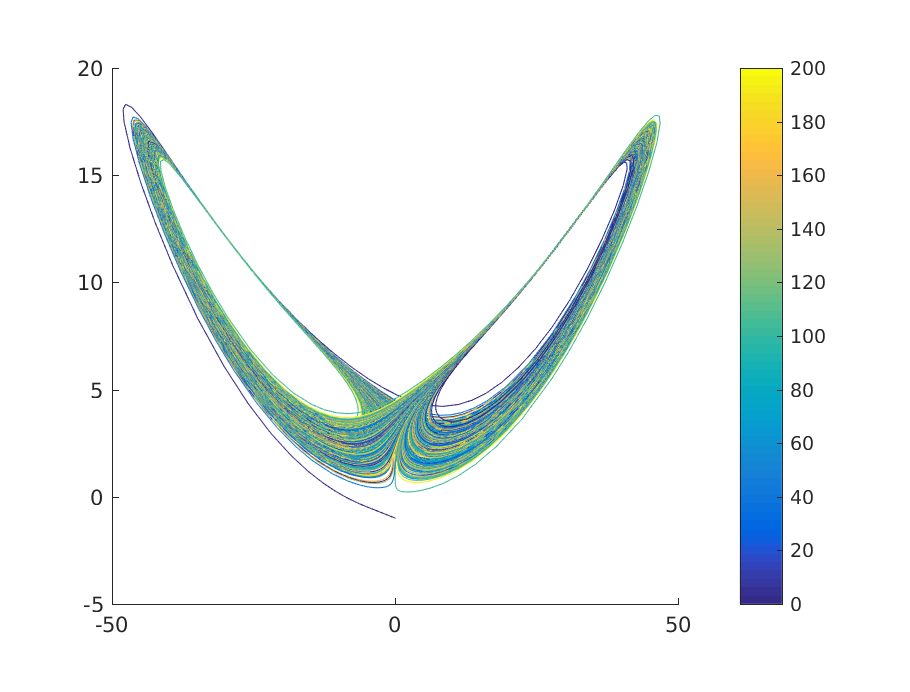
\includegraphics[width=\textwidth]{pictures/tercera_simulacion_xz}
		\caption{Vista XZ de la tercera simulación}
		\label{fig:simulacion3xz}
	\end{subfigure}

        \begin{subfigure}[b]{0.36\textwidth}
		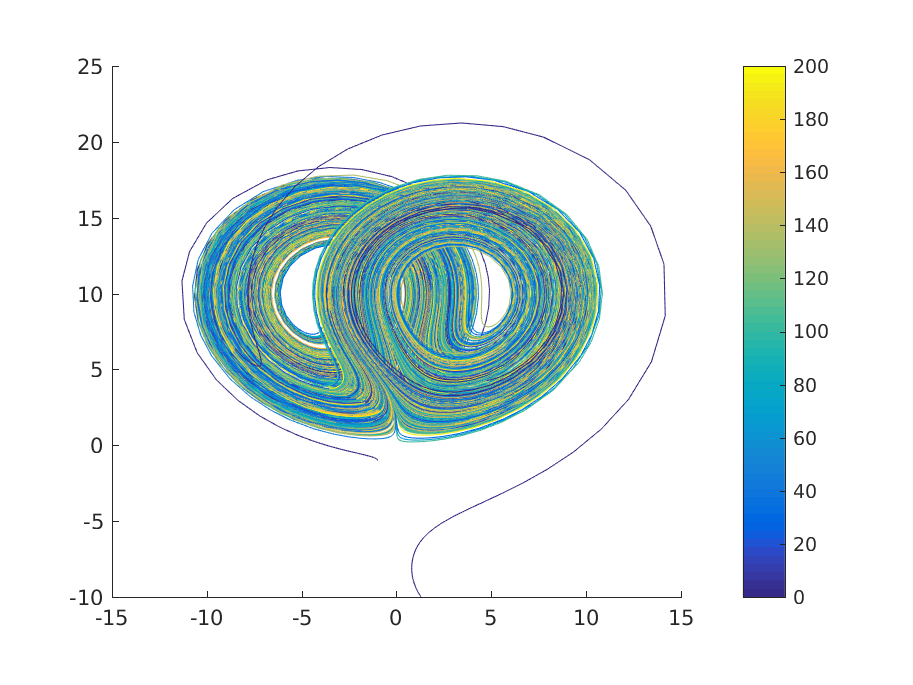
\includegraphics[width=\textwidth]{pictures/tercera_simulacion_yz}
		\caption{Vista YZ de la tercera simulación}
		\label{fig:simulacion3yz}
	\end{subfigure}
	\caption{Tercera simulación gráfica de los estados. En los ejes se tienen los estados y el tiempo se denota con el cambio de color}
	\label{fig:simulacion3_total}
\end{figure}

%Comparacion de los estados de las distintas simulaciones respecto al tiempo.···················································································

\begin{figure}
	\centering
	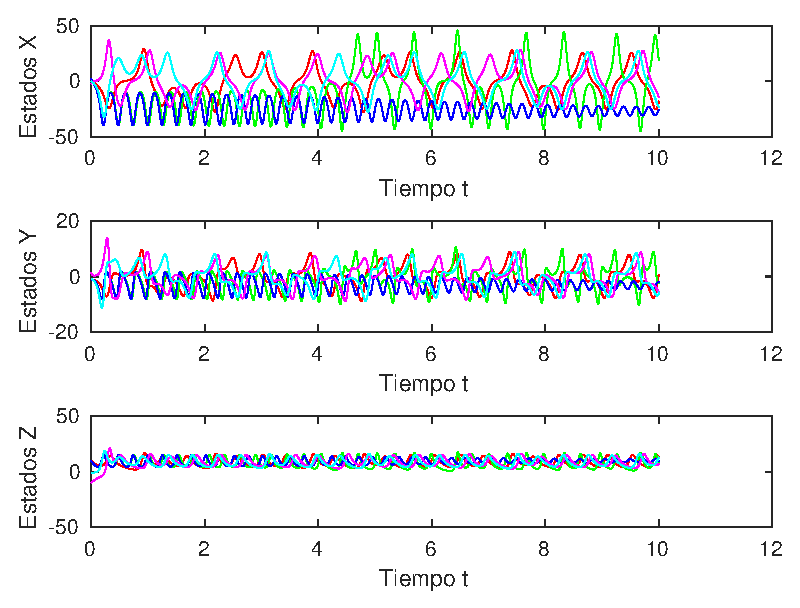
\includegraphics[width=\textwidth]{pictures/comparacion}
	\caption{Comparación de los estados de las distintas simulaciones respecto al tiempo}
	\label{fig:comparacion}
\end{figure}



\subsubsection{Código de ejercicio 1}



\section{Ejercicio 2}


\subsection{Código de ejercicio 2}

\section{Ejercicio 3}

\subsection{Código de ejercicio 3}

\end{document}
